\subsubsection{Dinámica de robot serie de 2 GDL}
Para el análisis dinámico de la estructura multiarticular de 2 grados de libertad (2-GDL), se emplea la formulación de Euler-Lagrange. Este método energético resulta particularmente eficiente para sistemas de cuerpos rígidos articulados, ya que evita el cálculo explícito de fuerzas de reacción internas y permite obtener directamente las ecuaciones de movimiento en términos de las coordenadas generalizadas.

El lagrangiano del sistema se define como:
\begin{equation}
\mathcal{L} = K - U
\end{equation}
donde $K$ es la energía cinética total y $U$ es la energía potencial total del sistema.

Las ecuaciones de movimiento se obtienen mediante las ecuaciones de Euler-Lagrange:
\begin{equation}
\tau_i = \frac{d}{dt}\left(\frac{\partial \mathcal{L}}{\partial \dot{\theta}_i}\right) - \frac{\partial \mathcal{L}}{\partial \theta_i}
\end{equation}
donde $\tau_i$ representa el torque aplicado en la articulación $i$ y $\theta_i$ son las coordenadas generalizadas (ángulos de rotación).


El sistema consiste en dos eslabones rígidos conectados en serie mediante articulaciones rotacionales. La configuración y parámetros se describen a continuación:
\begin{itemize}
    \item $L_1$: Longitud total del eslabón 1
    \item $L_2$: Longitud total del eslabón 2
    \item $l_1$: Distancia desde la articulación 1 al centro de masa del eslabón 1
    \item $l_2$: Distancia desde la articulación 2 al centro de masa del eslabón 2
    \item $m_1$, $m_2$: Masas de los eslabones 1 y 2
    \item $I_1$, $I_2$: Momentos de inercia de los eslabones respecto a sus centros de masa
\end{itemize}

\textbf{Coordenadas generalizadas:}
\begin{itemize}
    \item $\theta_1$: Ángulo de rotación de la articulación 1 (respecto al eje horizontal)
    \item $\theta_2$: Ángulo de rotación de la articulación 2 (respecto al eje horizontal)
\end{itemize}
\begin{figure}[H]
    \centering
    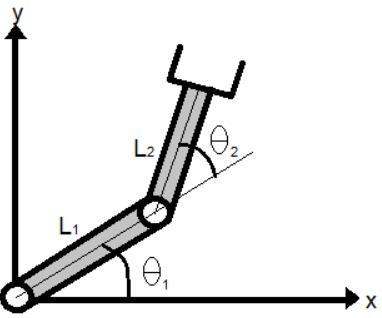
\includegraphics[width=0.65\textwidth]{img/DCL_brazo.png}
    \caption{\textit{Diagrama cinemático y de eslabones del manipulador robótico planar}}
    \label{fig:DCL_brazo}
\end{figure}
\paragraph{Energías del Eslabón 1}

\subparagraph{Energía Potencial}

La energía potencial gravitacional del eslabón 1 está dada por:
\begin{equation}
U_1 = m_1 \cdot g \cdot l_1 \cdot \sin(\theta_1)
\end{equation}

donde $g$ es la aceleración de la gravedad y la altura del centro de masa se mide desde un nivel de referencia horizontal.

\subparagraph{Energía Cinética}

La energía cinética del eslabón 1 tiene dos componentes: rotacional y traslacional.
\begin{equation}
K_1 = \frac{1}{2} I_1 \dot{\theta}_1^2 + \frac{1}{2} m_1 v_1^2
\end{equation}

Para calcular $v_1^2$, determinamos primero la posición del centro de masa del eslabón 1:
\begin{align}
x_1 &= l_1 \cos(\theta_1) \\
y_1 &= l_1 \sin(\theta_1)
\end{align}

Derivando respecto al tiempo:
\begin{align}
\dot{x}_1 &= -l_1 \sin(\theta_1) \dot{\theta}_1 \\
\dot{y}_1 &= l_1 \cos(\theta_1) \dot{\theta}_1
\end{align}

La velocidad al cuadrado del centro de masa es:
\begin{equation}
v_1^2 = \dot{x}_1^2 + \dot{y}_1^2 = l_1^2\sin^2(\theta_1)\dot{\theta}_1^2 + l_1^2\cos^2(\theta_1)\dot{\theta}_1^2 = l_1^2\dot{\theta}_1^2
\end{equation}

Por lo tanto, la energía cinética del eslabón 1 queda:
\begin{equation}
K_1 = \frac{1}{2}(m_1l_1^2 + I_1)\dot{\theta}_1^2
\end{equation}

\paragraph{Energías del eslabón 2}

\subparagraph{Energía potencial}

La energía potencial del eslabón 2 considera la altura de su centro de masa, que depende de ambos ángulos:
\begin{equation}
U_2 = m_2 \cdot g \cdot (L_1 \sin(\theta_1) + l_2 \sin(\theta_2))
\end{equation}

El primer término representa la contribución de la articulación 1, mientras que el segundo término corresponde a la posición del centro de masa del eslabón 2 respecto a la articulación 2.

\subparagraph{Energía cinética}

La energía cinética del eslabón 2 es:
\begin{equation}
K_2 = \frac{1}{2} I_2 \dot{\theta}_2^2 + \frac{1}{2} m_2 v_2^2
\end{equation}

La posición del centro de masa del eslabón 2 es:
\begin{align}
x_2 &= L_1\cos(\theta_1) + l_2\cos(\theta_2) \\
y_2 &= L_1\sin(\theta_1) + l_2\sin(\theta_2)
\end{align}

Derivando respecto al tiempo:
\begin{align}
\dot{x}_2 &= -L_1\sin(\theta_1)\dot{\theta}_1 - l_2\sin(\theta_2)\dot{\theta}_2 \\
\dot{y}_2 &= L_1\cos(\theta_1)\dot{\theta}_1 + l_2\cos(\theta_2)\dot{\theta}_2
\end{align}

Reemplazando x e y y sus derivadas se puede obtener $v_2^2$:
%\begin{multline}
%v_2^2 = \dot{x}_2^2 + \dot{y}_2^2 = (L_1\sin(\theta_1)\dot{\theta}_1 + l_2\sin(\theta_2)\dot{\theta}_2)^2 + (L_1\cos(\theta_1)\dot{\theta}_1 + l_2\cos(\theta_2)\dot{\theta}_2)^2
%\end{multline}

%Expandiendo:
%\begin{multline}
%v_2^2 = L_1^2\sin^2(\theta_1)\dot{\theta}_1^2 + l_2^2\sin^2(\theta_2)\dot{\theta}_2^2 + 2L_1l_2\sin(\theta_1)\sin(\theta_2)\dot{\theta}_1\dot{\theta}_2 \\
%+ L_1^2\cos^2(\theta_1)\dot{\theta}_1^2 + l_2^2\cos^2(\theta_2)\dot{\theta}_2^2 + 2L_1l_2\cos(\theta_1)\cos(\theta_2)\dot{\theta}_1\dot{\theta}_2
%\end{multline}

%Agrupando términos y aplicando la identidad trigonométrica $\sin^2(\alpha) + \cos^2(\alpha) = 1$:
%\begin{equation}
%v_2^2 = L_1^2\dot{\theta}_1^2 + l_2^2\dot{\theta}_2^2 + 2L_1l_2\dot{\theta}_1\dot{\theta}_2[\sin(\theta_1)\sin(\theta_2) + \cos(\theta_1)\cos(\theta_2)]
%\end{equation}

%Utilizando la identidad del coseno de la diferencia:
%\begin{equation}
%\cos(\theta_1 - \theta_2) = \cos(\theta_1)\cos(\theta_2) + \sin(\theta_1)\sin(\theta_2)
%\end{equation}
\begin{equation}
v_2^2 = L_1^2\dot{\theta}_1^2 + l_2^2\dot{\theta}_2^2 + 2L_1l_2\dot{\theta}_1\dot{\theta}_2\cos(\theta_1 - \theta_2)
\end{equation}

Por lo tanto, la energía cinética del eslabón 2 es:
\begin{equation}
K_2 = \frac{1}{2}I_2\dot{\theta}_2^2 + \frac{1}{2}m_2\left[L_1^2\dot{\theta}_1^2 + l_2^2\dot{\theta}_2^2 + 2L_1l_2\dot{\theta}_1\dot{\theta}_2\cos(\theta_1 - \theta_2)\right]
\end{equation}

El lagrangiano total del sistema es:
\begin{equation}
\mathcal{L} = K_1 + K_2 - U_1 - U_2
\end{equation}

Sustituyendo las expresiones obtenidas y simplificando se tiene:
%\begin{multline}
%\mathcal{L} = \frac{1}{2}(m_1l_1^2 + I_1)\dot{\theta}_1^2 + \frac{1}{2}(m_2l_2^2 + I_2)\dot{\theta}_2^2 + \frac{1}{2}m_2L_1^2\dot{\theta}_1^2 \\
%+ m_2L_1l_2\dot{\theta}_1\dot{\theta}_2\cos(\theta_1 - \theta_2) \\
%- m_1gl_1\sin(\theta_1) - m_2g[L_1\sin(\theta_1) + l_2\sin(\theta_2)]
%\end{multline}

%Simplificando:
\begin{multline}
\mathcal{L} = \frac{1}{2}(m_1l_1^2 + m_2L_1^2 + I_1)\dot{\theta}_1^2 + \frac{1}{2}(m_2l_2^2 + I_2)\dot{\theta}_2^2 + m_2L_1l_2\dot{\theta}_1\dot{\theta}_2\cos(\theta_1 - \theta_2) \\
- g[(m_1l_1 + m_2L_1)\sin(\theta_1) + m_2l_2\sin(\theta_2)]
\end{multline}

\paragraph{Para la coordenada $\theta_1$}

%Se calculan las derivadas parciales necesarias para la ecuación de Euler-Lagrange:

%\begin{equation}
%\frac{\partial \mathcal{L}}{\partial \dot{\theta}_1} = (m_1l_1^2 + m_2L_1^2 + I_1)\dot{\theta}_1 + m_2L_1l_2\dot{\theta}_2\cos(\theta_1 - \theta_2)
%\end{equation}

%Derivando respecto al tiempo:
\begin{multline}
\frac{d}{dt}\left(\frac{\partial \mathcal{L}}{\partial \dot{\theta}_1}\right) = (m_1l_1^2 + m_2L_1^2 + I_1)\ddot{\theta}_1 + m_2L_1l_2\ddot{\theta}_2\cos(\theta_1 - \theta_2) - m_2L_1l_2\dot{\theta}_2\sin(\theta_1 - \theta_2)(\dot{\theta}_1 - \dot{\theta}_2)
\end{multline}

%Derivada parcial respecto a $\theta_1$:
\begin{equation}
\frac{\partial \mathcal{L}}{\partial \theta_1} = -m_2L_1l_2\dot{\theta}_1\dot{\theta}_2\sin(\theta_1 - \theta_2) - g(m_1l_1 + m_2L_1)\cos(\theta_1)
\end{equation}

\paragraph{Para la coordenada $\theta_2$}

%\begin{equation}
%\frac{\partial \mathcal{L}}{\partial \dot{\theta}_2} = (m_2l_2^2 + I_2)\dot{\theta}_2 + m_2L_1l_2\dot{\theta}_1\cos(\theta_1 - \theta_2)
%\end{equation}

%Derivando respecto al tiempo:
\begin{multline}
\frac{d}{dt}\left(\frac{\partial \mathcal{L}}{\partial \dot{\theta}_2}\right) = (m_2l_2^2 + I_2)\ddot{\theta}_2 + m_2L_1l_2\ddot{\theta}_1\cos(\theta_1 - \theta_2) - m_2L_1l_2\dot{\theta}_1\sin(\theta_1 - \theta_2)(\dot{\theta}_1 - \dot{\theta}_2)
\end{multline}

%Derivada parcial respecto a $\theta_2$:
\begin{equation}
\frac{\partial \mathcal{L}}{\partial \theta_2} = m_2L_1l_2\dot{\theta}_1\dot{\theta}_2\sin(\theta_1 - \theta_2) - gm_2l_2\cos(\theta_2)
\end{equation}

Aplicando las ecuaciones de Euler-Lagrange $\tau_i = \frac{d}{dt}\left(\frac{\partial \mathcal{L}}{\partial \dot{\theta}_i}\right) - \frac{\partial \mathcal{L}}{\partial \theta_i}$, se obtienen los torques requeridos en cada articulación:

\paragraph{Torque en la articulación 1}

%\begin{multline}
%\tau_1 = (m_1l_1^2 + m_2L_1^2 + I_1)\ddot{\theta}_1 + m_2L_1l_2\ddot{\theta}_2\cos(\theta_1 - \theta_2) - m_2L_1l_2\dot{\theta}_2\sin(\theta_1 - \theta_2)(\dot{\theta}_1 - \dot{\theta}_2) \\
%+ m_2L_1l_2\dot{\theta}_1\dot{\theta}_2\sin(\theta_1 - \theta_2) + g(m_1l_1 + m_2L_1)\cos(\theta_1)
%\end{multline}

%Simplificando los términos de Coriolis:
\begin{multline}
\tau_1 = (m_1l_1^2 + m_2L_1^2 + I_1)\ddot{\theta}_1 + m_2L_1l_2\ddot{\theta}_2\cos(\theta_1 - \theta_2) - m_2L_1l_2\dot{\theta}_2^2\sin(\theta_1 - \theta_2) + g(m_1l_1 + m_2L_1)\cos(\theta_1)
\label{ec:torqueT1}
\end{multline}

\paragraph{Torque en la Articulación 2}

\begin{multline}
\tau_2 = (m_2l_2^2 + I_2)\ddot{\theta}_2 + m_2L_1l_2\ddot{\theta}_1\cos(\theta_1 - \theta_2) + m_2L_1l_2\dot{\theta}_1^2\sin(\theta_1 - \theta_2) + gm_2l_2\cos(\theta_2)
\label{ec:torqueT2}
\end{multline}

\subsubsection{Forma Matricial de las Ecuaciones}

Las ecuaciones de movimiento pueden expresarse en forma matricial compacta:
\begin{equation}
\mathbf{M}(\boldsymbol{\theta})\ddot{\boldsymbol{\theta}} + \mathbf{C}(\boldsymbol{\theta}, \dot{\boldsymbol{\theta}})\dot{\boldsymbol{\theta}} + \mathbf{G}(\boldsymbol{\theta}) = \boldsymbol{\tau}
\end{equation}

donde:
\begin{itemize}
    \item $\mathbf{M}(\boldsymbol{\theta})$ es la matriz de inercia (simétrica y definida positiva)
    \item $\mathbf{C}(\boldsymbol{\theta}, \dot{\boldsymbol{\theta}})$ contiene los términos de Coriolis y centrífugos
    \item $\mathbf{G}(\boldsymbol{\theta})$ es el vector de términos gravitacionales
    \item $\boldsymbol{\tau} = [\tau_1, \tau_2]^T$ es el vector de torques aplicados
\end{itemize}

\textbf{Matriz de Inercia:}
\begin{equation}
\mathbf{M} = \begin{bmatrix}
m_1l_1^2 + m_2L_1^2 + I_1 & m_2L_1l_2\cos(\theta_1 - \theta_2) \\
m_2L_1l_2\cos(\theta_1 - \theta_2) & m_2l_2^2 + I_2
\end{bmatrix}
\end{equation}

\textbf{Vector de Coriolis y centrífugos:}
\begin{equation}
\mathbf{C}\dot{\boldsymbol{\theta}} = \begin{bmatrix}
-m_2L_1l_2\sin(\theta_1 - \theta_2)\dot{\theta}_2^2 \\
m_2L_1l_2\sin(\theta_1 - \theta_2)\dot{\theta}_1^2
\end{bmatrix}
\end{equation}

\textbf{Vector gravitacional:}
\begin{equation}
\mathbf{G} = \begin{bmatrix}
-g(m_1l_1 + m_2L_1)\cos(\theta_1) \\
-gm_2l_2\cos(\theta_2)
\end{bmatrix}
\end{equation}

Las ecuaciones obtenidas presentan las siguientes características físicas relevantes:

\begin{enumerate}
    \item \textbf{Acoplamiento dinámico}: Los términos fuera de la diagonal en la matriz de inercia ($m_2L_1l_2\cos(\theta_1 - \theta_2)$) indican que el movimiento de una articulación afecta directamente a la otra. Este acoplamiento es más fuerte cuando los eslabones están alineados ($\theta_1 \approx \theta_2$) y se debilita cuando son perpendiculares. 
    \item \textbf{Efectos centrífugos}: Los términos proporcionales a $\dot{\theta}_i^2$ representan fuerzas centrífugas que dependen de las velocidades angulares al cuadrado.
    \item \textbf{Efectos de Coriolis}: Los términos de acoplamiento entre velocidades reflejan las fuerzas de Coriolis que surgen cuando ambas articulaciones se mueven simultáneamente.
    \item \textbf{Efectos gravitacionales}: Los términos gravitacionales son proporcionales al coseno de los ángulos, lo que indica que el torque gravitacional es máximo cuando los eslabones están horizontales y nulo cuando están verticales.
\end{enumerate}

